\documentclass[11pt]{article}
\usepackage[T1]{fontenc}
\usepackage{lmodern}
\usepackage[a4paper,margin=2.5cm]{geometry}
\usepackage{microtype}
\usepackage{amsmath,amssymb,mathtools,bm}
\usepackage{graphicx}
\usepackage{booktabs,tabularx,multirow,longtable,array}
\usepackage{enumitem}
\usepackage[dvipsnames]{xcolor}
\usepackage{tikz}
\usetikzlibrary{arrows.meta,positioning,shapes.geometric,fit,calc,backgrounds}
\usepackage{tcolorbox}
\usepackage{caption,subcaption}
\usepackage{float}
\usepackage[numbers,sort&compress]{natbib}
\usepackage[colorlinks=true,linkcolor=MidnightBlue,citecolor=MidnightBlue,urlcolor=MidnightBlue]{hyperref}
\usepackage[capitalise,noabbrev]{cleveref}
\usepackage{fancyhdr}
\pagestyle{fancy}\fancyhf{}\rhead{\small Strategy investigation by a distilled small agent}\lhead{\small Saadallah \& Jennane}\cfoot{\thepage}
\renewcommand{\headrulewidth}{0.3pt}
\setlist{itemsep=2pt,topsep=4pt}
\definecolor{accent}{HTML}{2F5BD3}
\definecolor{support}{HTML}{0F7B6C}
\definecolor{against}{HTML}{C2410C}
\newtheorem{definition}{Definition}
\newtheorem{proposition}{Proposition}
\newtheorem{remark}{Remark}
% A small algorithm box (the algorithm packages are not installed)
\newcounter{algo}
\newenvironment{algo}[1]{\refstepcounter{algo}\begin{tcolorbox}[colback=white,colframe=accent!70,boxrule=0.6pt,arc=2pt,left=6pt,right=6pt,top=4pt,bottom=4pt,
  title={\textbf{Algorithm \thealgo.} #1},fonttitle=\small,coltitle=white,colbacktitle=accent!85]\small}{\end{tcolorbox}}
\newcommand{\kw}[1]{\textbf{#1}}
\newcommand{\Tool}[1]{\texttt{#1}}
\newcommand{\E}{\mathbb{E}}
\setlength{\emergencystretch}{3em}


\title{\textbf{aemon: Teaching a Small Model to Investigate Strategy Questions}\\[4pt]
\large Agentic distillation of theory-driven decision making into a 3B open model,\\ with an executable environment and a frozen, blind evaluation}
\author{Hatem Saadallah \and Nour Jennane}
\date{November 2026}

\begin{document}
\maketitle
\thispagestyle{empty}

\begin{abstract}
\noindent Asked whether a manufacturer should take its technology to a new kind of customer, language models tend to
produce consulting prose rather than an investigation. We teach a small open model, Tiny Aya Global (3.35B parameters),
to carry out a theory-driven investigation (we call the resulting agent aemon; \emph{weigh what is known, test what is not}): frame the decision, state rival causal theories, weigh quoted evidence for
and against each, challenge its favourite, design a test with a decision rule or decline one, and revise on new
evidence. The procedure follows the scientific approach to strategic decisions, which treats a theory as a restriction on
beliefs and a decision as a choice between committing and experimenting. We build an executable environment with twelve
guarded tools over 1{,}334 verified public records, a stage controller and executable checks; distil 3{,}891 tool-call
rows from 158 replay-exact investigations by a Command A+ teacher into a LoRA adapter with AgentTune, plus 51 correction
rows; verify the deployed GGUF adapter against the trained one; and evaluate on four companies never used for training
or selection with two qualified, blinded LLM judges under a plan frozen before the run. The fine-tuned model scores 1.48
against 0.65 for the base model under its best prompt on a nine-dimension 0--3 rubric, a paired difference of $+0.83$
(95\% case-cluster bootstrap interval $[0.69, 0.97]$), higher for every company and every kind of new evidence, and
finishes 28 of 48 investigations against 4, at about \$0.03 per investigation against \$0.25 for Claude Opus. The final
system adds a second adapter and decoding-time guards that remove failing actions: it finishes 46 of 48 investigations
with 39 tool calls each (the base model needs 242), and the guards add $+0.12$ and $+0.21$ in judged quality on the two
test sets. A diagnosis
traces the remaining failures (no declined tests, little directional new evidence, decision rules cut by a length cap)
to gaps in the training data, and we report what environment changes and targeted examples did and did not fix.
\end{abstract}

\tableofcontents
\newpage

\section{Introduction}\label{sec:intro}

Ask a language model whether a manufacturer should take its technology to a new kind of customer, say whether a maker
of professional laundry machines should build something for households, and it will usually answer with consulting
prose: a list of factors, a confident market size with no source, and evidence collected only for the answer it started
with. Good strategy work looks different. It frames the decision and its real alternatives, including doing nothing;
it states rival theories of \emph{who} would change their behaviour and \emph{why}; it derives predictions that tell
those theories apart; it weighs quoted evidence for and against each and looks hardest for evidence against its
favourite; when information is worth its cost it proposes a test with a decision rule fixed in advance; and it revises
when new evidence arrives \citep{camuffo2020scientific,camuffo2024theory}.

This paper asks whether that procedure can be \emph{taught} to a small open model that runs on a single GPU, by
distilling the tool-using investigations of a much larger model inside an environment that enforces the procedure's
form. Our answer is a qualified yes. On a frozen test of four companies never used for training or selection, the
fine-tuned 3.35-billion-parameter student (Tiny Aya Global with a LoRA adapter) scores 1.48 on a blind nine-dimension
rubric against 0.65 for the same base model under its best prompt, a paired difference of $+0.83$ with a 95\%
case-cluster bootstrap interval of $[0.69, 0.97]$, and it finishes 28 of 48 investigations against 4. An investigation
costs about \$0.03 of rented GPU time, against \$0.25 measured for Claude Opus on an earlier control run of the task.

\paragraph{Contributions.}
\begin{enumerate}
  \item \textbf{An executable investigation environment} (\cref{sec:env}): twelve guarded tools over a dossier of
        1{,}334 verified public records when version~1 was trained and first tested (1{,}958 now), a stage controller that offers only the tools of the current step, and
        executable checks. Quotes must match a source word for word, theories must give distinct causal explanations, and
        a simulated what-if result may change a belief but can never support a recommendation about real demand.
  \item \textbf{A distillation pipeline with provenance} (\cref{sec:data,sec:training}): a Command A+ teacher runs the
        same environment; only investigations that replay exactly and reach an accepted finish become training rows,
        each bound by hash to its teacher episode and weights; training uses AgentTune's distillation trainer with loss
        on the target tool call only, followed by a conversion gate that checks the deployed GGUF adapter against the
        trained one.
  \item \textbf{A pre-registered evaluation} (\cref{sec:eval,sec:results}): a held-out company split, two LLM judges
        each qualified on matched sound and flawed investigations, blinded packets with the key kept apart, a statistic
        and rule fixed before the run, and a final test run exactly once.
  \item \textbf{An honest diagnosis and iteration} (\cref{sec:diagnosis,sec:iteration}): where the agent still fails,
        why the training data explains it, and what environment changes and targeted teacher examples did and did not
        fix.
  \item \textbf{A usable product} (\cref{sec:app}): aemon, which runs the agent locally for people who are
        not analysts, with answer-first results, charts counted from the record, follow-up questions grounded in the
        investigation's sources, memory, attachments and PDF reports.
\end{enumerate}
All code, the model and the data are public.\footnote{Model:
\url{https://huggingface.co/HatemSaadallah/tiny-aya-global-strategy-agent}; data:
\url{https://huggingface.co/datasets/HatemSaadallah/strategy-agent-investigations}.}

\section{Related work}\label{sec:related}
\paragraph{Tool-using language agents.} Interleaving reasoning with actions \citep{yao2023react} and teaching models to
call tools \citep{schick2023toolformer} made language agents practical. Fine-tuning small models on agent trajectories
from stronger models improves their tool use \citep{chen2023fireact,zeng2023agenttuning}. Our setting differs in that the
task has no single correct answer: quality lies in the \emph{process} (framing, rival theories, evidence handling,
experiment design, revision), so the environment must enforce form and the evaluation must judge substance.

\paragraph{Distillation.} Knowledge distillation trains a small student on a larger teacher's outputs
\citep{hinton2015distilling}. We distil at the level of tool calls: each training row is the context the teacher saw and
the one call it made, with the loss on that call only, and with parameter-efficient adapters \citep{hu2022lora,peft}
trained through AgentTune \citep{agenttune} on TRL \citep{trl}.

\paragraph{Structured generation.} Constraining decoding to a schema guarantees well-formed calls
\citep{willard2023outlines}. We constrain each turn to the tools open at the current step and to identifiers that exist,
which removes a class of failures; we also found a cost, a length cap that cut fields mid-sentence (\cref{sec:diagnosis}).

\paragraph{LLM judges.} Strong models are useful but imperfect judges \citep{zheng2023judging}. We qualify each judge on
matched sound and flawed investigations before using it, blind every packet, and report both judges and their agreement.

\paragraph{Strategy as science.} \citet{camuffo2020scientific} found in a randomised trial with start-ups that founders
taught to treat decisions as theory-driven experiments made better decisions; \citet{camuffo2024theory} formalise a
theory as a restriction on beliefs. We take their procedure as the target behaviour (\cref{sec:theory}).

\section{Theory: decisions as tests of theories}\label{sec:theory}

\subsection{The scientific approach to strategy}
Our target behaviour comes from the scientific approach to entrepreneurial and strategic decisions
\citep{camuffo2020scientific,camuffo2024theory}. A decision maker facing an uncertain opportunity should (i) frame the
decision and its real alternatives, including doing nothing; (ii) state \emph{theories}: causal accounts of who would
change their behaviour and why; (iii) derive predictions that tell the theories apart; (iv) gather evidence for and
against each, looking hardest for evidence against the favoured one; (v) when information is worth its cost, run a test
with a decision rule fixed in advance; and (vi) revise when new evidence arrives. Field experiments with start-ups found
that founders trained this way made more accurate decisions, pivoting or terminating sooner when evidence contradicted
them \citep{camuffo2020scientific}.

\subsection{A theory as a restriction on beliefs}
\citet{camuffo2024theory} formalise a theory as a Bayesian network with a restriction. We follow their running example,
Luxottica deciding whether eyeglasses could become a fashion product.

\paragraph{Attributes and states.} An \emph{attribute} is a question with an uncertain answer. Two attributes define the
state space: can the firm design fashion eyewear ($Y$ or $N$), and will demand be high or low ($H$ or $L$). The four
states are $\{YH, YL, NH, NL\}$, and the decision maker cares about the probability of high demand,
\begin{equation}
  P(H) = \theta_Y\,\theta_{H|Y} + (1-\theta_Y)\,\theta_{H|N},
  \label{eq:ph}
\end{equation}
where $\theta_Y = P(Y)$, $\theta_{H|Y} = P(H\mid Y)$ and $\theta_{H|N} = P(H\mid N)$.

\paragraph{The theory.} The theory ``fashion design causes demand'' is one arrow $Y \to H$ in a Bayesian network together
with an inequality on its conditional probabilities,
\begin{equation}
  \Theta = \{\theta : \theta_{H|Y} > \theta_{H|N}\},
  \qquad
  \tilde\Theta = \{\theta : \theta_{H|Y} = \theta_{H|N}\},
\end{equation}
where $\tilde\Theta$ is the null hypothesis that design has no effect.

\paragraph{Value of a theory.} The parameters are unknown, so the decision maker holds a distribution $\mu$ over them. Let
$V_\Theta = \E_{\mu}[P(H)\mid\theta\in\Theta]$ and $V_{\tilde\Theta} = \E_{\mu}[P(H)\mid\theta\in\tilde\Theta]$. With prior
$\omega$ that the theory is right, its value is
\begin{equation}
  V = \omega\,V_\Theta + (1-\omega)\,V_{\tilde\Theta}.
  \label{eq:value}
\end{equation}

\paragraph{A worked example.} Take $\theta_{H|N}=0.5$ and $\theta_Y=0.8$ with probability one, and $\theta_{H|Y}$ uniform.
Under the theory $\theta_{H|Y}$ is uniform on $(0.5,1)$, so $\E[\theta_{H|Y}\mid\Theta]=0.75$ and
\begin{equation}
  V_\Theta = 0.8\cdot 0.75 + 0.2\cdot 0.5 = 0.70 .
\end{equation}
Without the restriction $\theta_{H|Y}$ averages $0.5$ and $P(H)=0.5$. The theory raises belief in high demand by
\emph{ruling parameter values out}: it is informative precisely because it can be wrong.

\paragraph{Experiments.} An experiment produces evidence that updates $\mu$, and with it $V_\Theta$ and
$V_{\tilde\Theta}$. In their account the prior on the theory itself changes only when the evidence moves the beliefs about
parameters far enough, $\lVert \mu' - \mu \rVert > \mu^*$: a small surprise adjusts parameters, a large one shakes belief in
the theory. A rival theory has its own value $Q$, built the same way. With costly experiments the decision maker should
commit once $V$ is far enough above or below $Q$, and experiment in between, the logic of optimal stopping for
costly information \citep{moscarini2001optimal}. Experiments are assumed Bayes plausible: before running one there is no
reason to expect it to move the value in a particular direction.

\begin{remark}[Bayesian updating, illustrated]\label{rem:bayes}
For intuition, suppose $n$ customers are shown the fashion design and $k$ buy. Under the theory, with
$\theta_{H|Y}\sim U(\theta_{H|N},1)$, and under the null, with $\theta_{H|Y}=\theta_{H|N}$, the marginal likelihoods are
\begin{equation}
  m_\Theta(k) = \frac{1}{1-\theta_{H|N}}\int_{\theta_{H|N}}^{1}\binom{n}{k}p^k(1-p)^{n-k}\,dp,
  \qquad
  m_{\tilde\Theta}(k) = \binom{n}{k}\theta_{H|N}^k(1-\theta_{H|N})^{n-k},
\end{equation}
and Bayes' rule gives the posterior on the theory
\begin{equation}
  \omega' = \frac{\omega\, m_\Theta(k)}{\omega\, m_\Theta(k) + (1-\omega)\, m_{\tilde\Theta}(k)}.
\end{equation}
Full updating moves $\omega$ after every observation; the threshold rule of \citet{camuffo2024theory} moves it only after
large surprises, so this calculation overstates how often a theory itself is revised.
\end{remark}

\subsection{From the framework to an agent}
The agent in this paper does \emph{not} compute these quantities, and neither does its environment. A computed update would
need an invented network and invented likelihoods, and assumed ratios could manufacture exactly the revision we want to
measure. Instead the agent carries out the framework's steps in words, with tools and quoted evidence, and the environment
enforces their form:
\begin{itemize}
  \item \emph{theories} are explicit causal claims (who benefits, why behaviour changes, how value is captured), and two of
        them must be genuinely distinct (\cref{sec:env});
  \item \emph{evidence} is a quoted passage from a source, assessed as supporting, contradicting or having no bearing on a
        theory, with what it does not show;
  \item \emph{tests} carry a prediction per theory and a decision rule, within a budget and a time limit;
  \item \emph{beliefs} are stated on a five-step verbal scale (very unlikely, unlikely, uncertain, likely, very likely)
        when the agent takes a position and again after new evidence. The scale is a within-run signal, not a calibrated
        probability; a direction check asks only whether undermining evidence did not raise the affected theory and
        supporting evidence did not lower it.
\end{itemize}
The framework thus supplies the \emph{grammar} of a good investigation; the environment makes that grammar executable;
and fine-tuning teaches a small model to speak it.

\section{The investigation environment}\label{sec:env}

\subsection{An investigation as a sequential decision problem}
We model one investigation as a finite-horizon sequential decision problem. A \emph{case} $c$ fixes a company, a
question, a brief, budgets and a dossier $D_c$ of public records the case may see. The state $s_t$ holds everything on
record at step $t$: the frame (objective, constraints, alternatives), the sources read, the theories, the assessed
quotes, any test or declined test, the stated position, revisions and the final answer. An action is one tool call
$a_t = (\textit{name}, \textit{arguments})$. A guarded transition $\mathcal{T}$ either accepts the call and updates the
state, or refuses it with a reason and leaves the state unchanged:
\begin{equation}
  (s_{t+1}, r_t) =
  \begin{cases}
    (\delta(s_t, a_t), \textit{result}) & \text{if every guard on } a_t \text{ holds in } s_t,\\
    (s_t, \textit{refusal}(\textit{category}, \textit{reason})) & \text{otherwise.}
  \end{cases}
\end{equation}
The agent never sees $s_t$ in full; it sees a compact observation $o_t = \phi(s_t)$ (\cref{sec:agent}). An episode ends
when the agent finishes, after $E$ refusals in a row ($E=4$ as evaluated), at a turn limit ($T=45$), or when the context
is full.

\subsection{Tools}
Staged runs expose twelve tools (\cref{tab:tools}). Each argument has an exact key set and length limits; a call with
missing or extra keys is refused.

\begin{table}[H]\centering\small
\caption{The twelve tools, their arguments and what makes them refuse a call.}\label{tab:tools}
\begin{tabularx}{\linewidth}{@{}>{\ttfamily}l X X@{}}
\toprule
\normalfont Tool & Arguments & Refused when (category)\\
\midrule
read\_brief & none & arguments given\\
frame\_problem & objective; 1--6 constraints; 2--6 alternatives & already framed (repeat); brief not read (order)\\
search\_evidence & query & no frame yet (order); no searches left, or the last one is reserved for the challenge (budget); same search again (repeat)\\
read\_source & id & the id never came from a search (fabricated)\\
add\_theory & claim, who benefits, why behaviour changes, how value is captured; assumptions; predictions & more than 5 theories (budget); identical claim (repeat)\\
assess\_evidence & theory, source, direction, quote, evidence kind, what it does not show & source not read (unread\_evidence); quote not in the source (misquote); a simulated source used as support (synthetic\_as\_evidence); same theory--source pair (repeat)\\
challenge\_theory & theory, query & unknown theory; budget; repeat\\
propose\_test & name, $\ge2$ theories, method, sample, measure, one prediction per theory, decision rule, cost, weeks & over the test budget or time limit (budget); arguments\\
decline\_test & reason & arguments\\
state\_position & favoured theory, recommendation, one belief per theory & favoured theory never challenged (order)\\
revise\_theory & theory, status (kept, revised, rejected), reason, new claim, evidence & cites unread evidence; a revised claim that does not change\\
finish & recommendation, target customer, value proposition, favoured theory, next action, uncertainty, what would change it, evidence; beliefs & cites unread evidence; cites a simulated record (synthetic\_as\_evidence)\\
\bottomrule
\end{tabularx}
\end{table}

\subsection{Guards}
\paragraph{Exact quotation.} An assessment's quote $q$ must appear in the source's excerpt $x$ after normalisation:
\begin{equation}
  \textit{valid}(q, x) \iff |q|_{\text{words}} \ge 3 \;\wedge\; |\nu(q)| \ge 15 \;\wedge\; \nu(q) \sqsubseteq \nu(x),
\end{equation}
where $\nu$ lowercases, collapses whitespace and maps curly quotes, dashes and non-breaking spaces to plain forms, and
$\sqsubseteq$ is substring containment. Surrounding quotation marks are stripped first: half of the teacher's early
refused quotes were exact words inside quotation marks.

\paragraph{Distinct theories.} Two theories are near-duplicates when the Jaccard similarity of their processed word sets
(claim plus why behaviour changes) reaches $\tau = 0.6$:
\begin{equation}
  J(A,B) = \frac{|A \cap B|}{|A \cup B|} \ge 0.6 .
\end{equation}
The tool refuses an identical claim; the executable check fails a run with any pair above the threshold.

\paragraph{Simulated evidence.} A what-if record is written by the case authors and starts with ``SIMULATED''. It may be
read and assessed as contradicting or neutral, and it may move a belief, but it may never support a theory or be cited
in the recommendation.

\subsection{The stage controller}
A controller $\mathcal{C}$ maps the state to the current step and the tools open in it, $A(s_t)$, and adds a one-line
instruction to every observation. \Cref{tab:stages} lists the steps and what moves each on. Decoding is constrained to
$A(s_t)$, so a call to a closed tool cannot be produced at all.

\begin{table}[H]\centering\small
\caption{Steps of the stage controller.}\label{tab:stages}
\begin{tabularx}{\linewidth}{@{}l X X@{}}
\toprule
Step & Open tools & Moves on when\\
\midrule
brief & read\_brief & the brief is read\\
frame & frame\_problem & a frame exists\\
evidence & search, read & 3 sources are read\\
theories & add\_theory, search, read & at least 2 theories exist\\
assessment & assess\_evidence, read, search, add\_theory & every theory has a weighed source\\
challenge & challenge\_theory & one search against a theory\\
challenge reading & read, challenge\_theory & what the challenge found has been read\\
test & propose\_test, decline\_test, and the look-further tools & a test is proposed or declined\\
position & state\_position, look-further tools & a position is stated (its favourite challenged)\\
new evidence & read & the what-if is read (cases with a what-if)\\
update & revise\_theory & a revision cites the what-if\\
conclude & finish, revise\_theory, look-further tools & the investigation finishes\\
\bottomrule
\end{tabularx}
\end{table}

\subsection{Search}
Search is deliberately plain. Terms are lower-case alphanumeric tokens with stop words removed and a crude plural
stripped. A record's score for a query $Q$ is the summed inverse document frequency of the shared terms,
\begin{equation}
  \textit{score}(r, Q) = \sum_{w \in Q \cap r} \log\!\Bigl(1 + \frac{N}{n_w}\Bigr),
\end{equation}
with $N$ records and $n_w$ containing $w$; the top three are returned. Each case allows 8 searches, the last reserved
for a challenge. Search knows nothing about theories, so finding evidence against a favourite is the agent's job.

\subsection{Executable checks}
Every finished or stopped run is checked mechanically. The checks include framing (at least three alternatives,
including no expansion or a different route), distinct theories, causal form (no ``should'' in a claim), testable
predictions, evidence use, evidence classes (no theory supported only by company claims or simulated results),
evidence limits, disconfirmation (the favourite was challenged and what was found was read), experiment design
(predictions that differ and a decision rule with a measurable threshold, or a decline where no test is warranted),
revision on new evidence, the existing offering (premise records read), no invented numbers, no simulated evidence in
the recommendation, a recommendation with a distinct next action and at least two sources, and at least 80\% of calls
accepted. The checks are guards against mechanical mistakes, not a measure of strategic quality; that is what the
judges are for (\cref{sec:eval}).

\subsection{Cases and the dossier}
When version~1 was trained and first tested the dossier held 1{,}334 public records (935 independent observations, 399
company claims; 1{,}958 now, with the second test's companies and later training cases), each with source, URL, date
and a short excerpt, every excerpt checked against its live source on the access date. Each case sees only its own
company's records (and, for three original cases, a shared market set). There were then 137 development cases on 64 companies (207 on 99 now):
for every company a base case and a variant in which an irrelevant simulated result arrives mid-investigation, and for
three companies also supporting and undermining what-ifs. Every case allows 8 searches, a test budget of 20{,}000 euros
and 12 weeks, which the brief calls analyst assumptions. Eighteen cases (nine companies) are marked as not warranting a
test, so declining is the right call there.

The split is by company, never by row: 58 training companies (122 cases), 6 validation companies (15 cases, used for
selection) and 4 test companies (16 cases: base, irrelevant, supporting and undermining for each of Aquaporin, Electrolux
Professional, RATIONAL and Simonelli), held in a separate file that development runs never load.

\section{The agent}\label{sec:agent}

\begin{figure}[t]\centering
\resizebox{0.92\linewidth}{!}{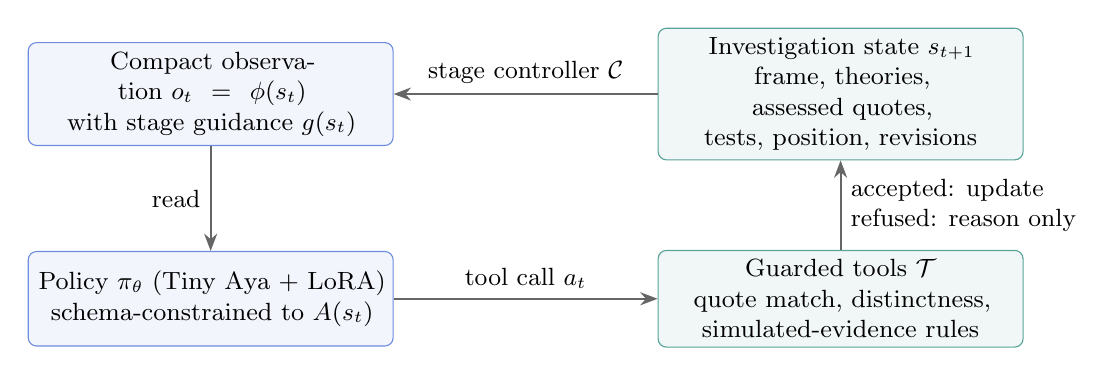
\begin{tikzpicture}[every node/.style={font=\small},
  box/.style={draw=accent!70, rounded corners=3pt, fill=accent!6, align=center, minimum height=12mm, text width=44mm},
  env/.style={draw=support!70, rounded corners=3pt, fill=support!6, align=center, minimum height=12mm, text width=44mm},
  arr/.style={-{Stealth[length=2.2mm]}, thick, draw=black!60}]
\node[box] (obs) at (0,0) {Compact observation $o_t=\phi(s_t)$\\with stage guidance $g(s_t)$};
\node[box] (policy) at (0,-2.6) {Policy $\pi_\theta$ (Tiny Aya + LoRA)\\schema-constrained to $A(s_t)$};
\node[env] (guard) at (8,-2.6) {Guarded tools $\mathcal{T}$\\quote match, distinctness,\\simulated-evidence rules};
\node[env] (state) at (8,0) {Investigation state $s_{t+1}$\\frame, theories, assessed quotes,\\tests, position, revisions};
\draw[arr] (obs) -- node[left]{read} (policy);
\draw[arr] (policy) -- node[above]{tool call $a_t$} (guard);
\draw[arr] (guard) -- node[right, align=left]{accepted: update\\refused: reason only} (state);
\draw[arr] (state) -- node[above]{stage controller $\mathcal{C}$} (obs);
\end{tikzpicture}
}
\caption{One step of an investigation. The policy reads a compact observation of the state, emits one tool call that
decoding restricts to the open tools, and the guarded tools either update the state or refuse with a reason.}
\label{fig:loop}
\end{figure}

\subsection{Policy and observation}
The policy $\pi_\theta$ is Tiny Aya Global \citep{tinyaya} (3.349 billion parameters, 36 layers, hidden size 2{,}048)
with a LoRA adapter. At each step it receives a fixed system prompt and one user message, the compact observation
\begin{equation}
  o_t = \phi(s_t) \oplus g(s_t) \oplus \textit{result}_{t-1},
\end{equation}
where $\phi$ serialises the state as it stands (the question, budgets, frame, unread search results, every source read
with its excerpt, the theories, every assessment, the challenge, tests, position, revisions and the last twelve tried
calls), $g$ is the controller's guidance (the step's instruction, its open tools and the searches left), and the last
tool result is appended. Guidance is added to what the model is shown, never to the record, so every recorded episode
replays exactly. The observation replaces a transcript: the model sees the state, not a history it could copy.

\subsection{Constrained decoding}
Each turn is decoded under a JSON schema $\Sigma(s_t)$ that admits exactly one call to a tool in $A(s_t)$, with
identifiers drawn from those that exist (theory ids, sources read) and length limits per field. The schema guarantees a
well-formed call; whether it is a \emph{good} call is the model's. As evaluated, short text fields were limited to 240
characters, which we later found cut test designs mid-sentence (\cref{sec:diagnosis}); the limits were raised to 900
for methods and decision rules and 500 for samples and measures afterwards.

\subsection{Sampling and stopping}
Decoding is greedy (temperature 0). Straight after a refused call the next attempt samples at temperature 0.4 with a
seed that depends on the case, the attempt and the number of refusals in a row,
\begin{equation}
  \textit{seed} = \sum_{ch \in \textit{case id}} \textit{ord}(ch) + 1000\,\textit{attempt} + \textit{errors},
\end{equation}
so a retry is not a repeat of the refused call. A run stops after 4 refusals in a row or 45 turns, with a context of
12{,}288 tokens and 520 tokens per turn.

\begin{algo}{One investigation (the evaluated runner)}\label{alg:run}
\kw{input:} case $c$, policy $\pi_\theta$, prompt $P$; \kw{limits:} $T=45$, $E=4$\\
$s \gets s_0(c)$; $e \gets 0$; $o \gets$ ``A new investigation is ready. Call read\_brief.''\\
\kw{for} $t = 1,\dots,T$ \kw{do}\\
\hspace*{1.2em} $\tau \gets 0$ \kw{if} $e = 0$ \kw{else} $0.4$\\
\hspace*{1.2em} $a \gets \textsc{Decode}(\pi_\theta, P, o;\ \Sigma(s), \tau, \textit{seed}(c, e))$ \hfill (schema-constrained)\\
\hspace*{1.2em} $(s', r) \gets \mathcal{T}(s, a)$\\
\hspace*{1.2em} \kw{if} $r$ is a refusal \kw{then} $e \gets e + 1$ \kw{else} $e \gets 0$; $s \gets s'$\\
\hspace*{1.2em} \kw{if} $s$ is finished \kw{then return} $s$, ``finished''\\
\hspace*{1.2em} \kw{if} $e \ge E$ \kw{then return} $s$, ``repeated errors''\\
\hspace*{1.2em} $o \gets \phi(s) \oplus g(s) \oplus r$\\
\kw{return} $s$, ``turn limit''
\end{algo}

\section{Training data from a teacher}\label{sec:data}

\begin{figure}[t]\centering
\resizebox{\linewidth}{!}{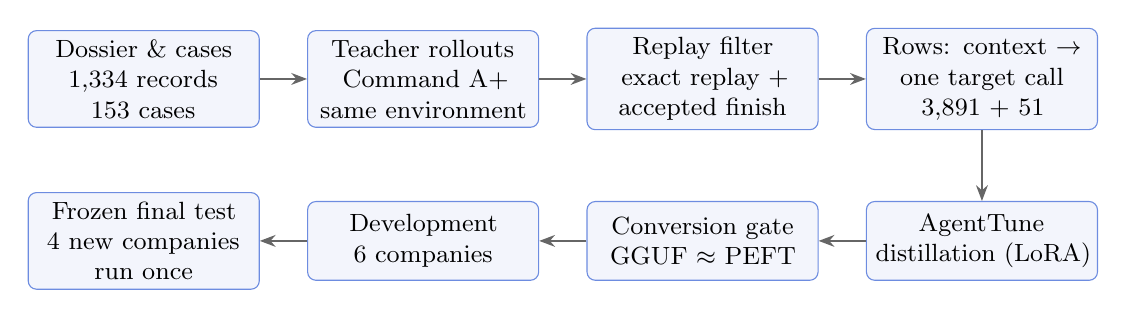
\begin{tikzpicture}[node distance=5mm and 6mm, every node/.style={font=\small},
  st/.style={draw=accent!70, rounded corners=3pt, fill=accent!6, align=center, minimum height=10mm, text width=27mm},
  arr/.style={-{Stealth[length=2mm]}, thick, draw=black!60}]
\node[st] (d) {Dossier \& cases\\1{,}334 records\\153 cases};
\node[st, right=of d] (t) {Teacher rollouts\\Command A+\\same environment};
\node[st, right=of t] (r) {Replay filter\\exact replay +\\accepted finish};
\node[st, right=of r] (rows) {Rows: context $\to$\\one target call\\3{,}891 + 51};
\node[st, below=9mm of rows] (sft) {AgentTune\\distillation (LoRA)};
\node[st, left=of sft] (gate) {Conversion gate\\GGUF $\approx$ PEFT};
\node[st, left=of gate] (dev) {Development\\6 companies};
\node[st, left=of dev] (fin) {Frozen final test\\4 new companies\\run once};
\draw[arr] (d) -- (t); \draw[arr] (t) -- (r); \draw[arr] (r) -- (rows); \draw[arr] (rows) -- (sft);
\draw[arr] (sft) -- (gate); \draw[arr] (gate) -- (dev); \draw[arr] (dev) -- (fin);
\end{tikzpicture}
}
\caption{From dossier to evaluation. Only exact, accepted teacher investigations become rows; the trained adapter must
pass the conversion gate before any evaluation; the final test runs once.}
\label{fig:pipeline}
\end{figure}

\subsection{The teacher}
The teacher is Command A+ \citep{commandaplus} (Apache 2.0), quantised to Q4\_K\_M and served with llama.cpp
\citep{llamacpp} on a single A100, with the same tools, controller and checks as the student and a teacher prompt that
adds rules for good practice. Claude was excluded as a teacher because its commercial terms bar using its outputs to
train a competing model; Aya Expanse 32B was tried first and rejected for weak reasoning.

\subsection{The replay filter}
A teacher investigation becomes training data only if it is \emph{exactly reproducible} and \emph{accepted}: replaying
its recorded turns through a fresh environment must reproduce every tool result and the recorded call sequence, and must
reach an accepted finish. Its provenance must match the permitted teacher weights in an append-only manifest. Passing the
executable checks is recorded but not required, because a teacher investigation can be instructive while failing a
check; the checks are reported, and the judges score quality.

\begin{algo}{Rows from teacher investigations}\label{alg:rows}
\kw{for each} teacher episode $\epsilon = (c, \{(a_t, r_t)\}_{t\le T})$ \kw{do}\\
\hspace*{1.2em} \kw{require} $\textit{hash}(\textit{weights}(\epsilon)) \in \textit{manifest}$ \kw{and} $\epsilon$ not excluded on review\\
\hspace*{1.2em} $s \gets s_0(c)$\\
\hspace*{1.2em} \kw{for} $t = 1,\dots,T$ \kw{do}\\
\hspace*{2.4em} $(s', r') \gets \mathcal{T}(s, a_t)$; \kw{require} $r' = r_t$ \hfill (exact replay)\\
\hspace*{2.4em} \kw{if} $a_t$ was accepted \kw{then} emit row $\bigl(x = P \oplus \phi(s) \oplus g(s) \oplus r_{t-1},\ y = a_t\bigr)$\\
\hspace*{2.4em} $s \gets s'$\\
\hspace*{1.2em} \kw{require} $s$ finished and the finish accepted; \kw{else} discard every row of $\epsilon$
\end{algo}

Refused calls never become targets. Each row is bound by hash to its teacher episode and weights. A row longer than
8{,}192 tokens is refused, never truncated; the longest kept row is 6{,}011 tokens.

\subsection{Counts}
174 teacher investigations passed the filter, giving 4{,}302 rows. Training used the 3{,}891 rows from 158
investigations on 57 training companies; the 411 rows on validation companies were kept for held-out loss only.

\subsection{Correction rows}
To teach recovery from loops, we harvested states from the student's own runs on training companies where a loop began
(a refused repeat, a third read of one source, or two refusals in a row; at most three per run) and asked the teacher
for the single best next call, preceded by what had been learned, what remained uncertain and why the call helps. A reply
was kept only if it was valid JSON, did not repeat an earlier call, was accepted by the tools, named something from the
state, and acted on what it named; in the test step it had to propose a test with distinct predictions and a numeric
rule or decline with a reason. 80 replies were provisionally kept and 51 became rows (49 at the theories step, one
assessment, one conclusion), 0.35\% of supervised tokens.

\section{Training}\label{sec:training}

\subsection{Objective}
Each row is a context $x$ and a target call $y = (y_1,\dots,y_m)$. The student is trained by supervised distillation with
the loss on the target tokens only:
\begin{equation}
  \mathcal{L}(\theta) = -\frac{1}{\sum_i m_i}\sum_{i}\sum_{j=1}^{m_i} \log \pi_\theta\bigl(y^{(i)}_j \mid x^{(i)}, y^{(i)}_{<j}\bigr),
\end{equation}
implemented by giving every context token the label $-100$; the context's tokens must be an exact prefix of the full
row's tokens, or the build fails. This is sequence-level distillation from the teacher's chosen calls
\citep{hinton2015distilling}.

\subsection{Parameter-efficient adaptation}
Every linear layer $W_0 \in \mathbb{R}^{d\times k}$ in attention and MLP blocks is adapted with a low-rank update
\citep{hu2022lora},
\begin{equation}
  W = W_0 + \frac{\alpha}{r} B A, \qquad B \in \mathbb{R}^{d\times r},\; A \in \mathbb{R}^{r\times k},
\end{equation}
with rank $r = 16$, $\alpha = 32$ and dropout 0.05; $W_0$ is frozen. The adapter has 504 tensors (about 121 MB).

\subsection{Procedure and settings}
Training used AgentTune's distillation trainer \citep{agenttune} with a TRL supervised trainer \citep{trl} and PEFT
\citep{peft}. Settings: 2 epochs; learning rate $1\times10^{-4}$ with 5\% linear warmup and cosine decay; batch size 1
with gradient accumulation 4 (effective batch 4); maximum length 8{,}192 tokens; bf16; seed 7. On the 3{,}942 training
rows (3{,}891 teacher rows and 51 corrections) this is $3942 \times 2 / 4 = 1{,}971$ optimiser steps. Validation loss is
the unweighted mean over validation companies of up to 40 evenly spaced rows each, so no company dominates; the best
checkpoint by validation loss is kept. An overfit gate runs first: 10 rows for 60 steps must be reproduced greedily in
at least 8 of 10 cases, or training stops. Training ran on a 40 GB slice of an A100 on a university cluster. The final
held-out loss was 0.7125, at the last checkpoint.

\subsection{The conversion gate}
The trained PEFT adapter is converted to GGUF for llama.cpp, and a conversion can silently change behaviour. Before any
evaluation, the gate replays recorded points of real investigations and compares, over the full vocabulary of 262{,}144
tokens, the converted adapter's effect on the next-token distribution with the PEFT adapter's effect,
\begin{equation}
  \Delta_{\text{PEFT}} = \log p_{\text{base+LoRA}} - \log p_{\text{base}}, \qquad
  \Delta_{\text{GGUF}} = \log q_{\text{base+LoRA}} - \log q_{\text{base}},
\end{equation}
passing when the cosine similarity of the two effects is at least 0.99 and the probability-weighted residual RMS is at
most 0.15 at every point, and a tensor audit confirms the factor pairs were cast as expected. Comparing \emph{effects}
rather than absolute log-probabilities matters: the base model alone differs by up to 0.19 between the two backends, which
made an earlier absolute-gap gate fail for reasons that had nothing to do with the adapter. The final adapter passed on
11 points with minimum cosine 0.9990 and maximum residual 0.080; the file evaluated is byte-identical to the one gated
(sha256 41794b57\ldots).

\section{Evaluation design}\label{sec:eval}

\subsection{What is measured}
The primary outcome is \emph{investigation quality} as judged blind against a frozen rubric of nine dimensions, each
scored 0 to 3 (\cref{tab:rubric}). A judge gives the highest rung whose conditions are all met; an invented number,
customer or company intention caps that dimension at 1. Dimensions the run never reached score 0; dimensions that do not
apply (revision when no new evidence arrived) are excluded. An episode's score is the mean over its scored dimensions.

\begin{table}[H]\centering\footnotesize
\caption{The rubric (abridged). Scores 0 to 3.}\label{tab:rubric}
\begin{tabularx}{\linewidth}{@{}l X X@{}}
\toprule
Dimension & 2 & 3\\
\midrule
Problem framing & separates the objective from the suggested solution & also finds an option or constraint a good analyst would not want missed, or corrects a false premise\\
Causal mechanism & who changes behaviour and why & the full chain from behaviour change to value this manufacturer captures\\
Distinct theories & rival explanations of the same question & rivals implying different products, customers or channels\\
Assumptions and predictions & observable & observable, and the theory is in trouble if they fail\\
Evidence judgement & separates company assertions, observations, studies and analogies & says what each key source cannot establish\\
Seeking challenge & genuinely searches against its favourite & reports fairly what it found, including nothing\\
Experiment design & separates at least two theories, or soundly declines & also feasible and decision-relevant\\
Revision & a proportionate, evidence-linked response to the affected theory & also traces the implications without overreacting\\
Recommendation & follows from the evidence, with stated uncertainty & commits to a next action and says what would reverse it\\
\bottomrule
\end{tabularx}
\end{table}

\subsection{Judges and their qualification}
Two LLM judges score every packet: Claude (Opus 5.5, 8{,}000 output tokens, medium effort) and Codex (GPT-6-astra
through its command-line tool, with shell, web, memory and repository access disabled). Before use, each was
\emph{qualified} on 20 matched pairs of fictional investigations, one sound and one deliberately flawed in each pair,
under a rule registered before it was computed: the sound version must score strictly higher in at least 17 of 20
pairs, with ties and invalid outputs counted as failures, and at most 4 of 40 outputs invalid after one retry. Claude
passed 20 of 20 at 8{,}000 tokens (19 of 20 at 3{,}000, with one truncated output, which led to the higher limit);
Codex passed 20 of 20. A caveat: Codex wrote the qualification packets and their key.

\subsection{Blinding}
A packet shows the investigation as a reader would see it, with no arm, model, adapter, prompt or run name; refused
calls are omitted and identical consecutive calls are shown once with a count. Packet ids are content hashes, the order
is shuffled with a fixed seed (20261106), and the key linking packets to arms is kept outside the repository while
judging.

\subsection{The statistic}
Let $q_{j,k}(c, a)$ be judge $j$'s score of arm $k$ on case $c$, attempt $a$. The paired difference for one
case and attempt, averaged over the two judges, is
\begin{equation}
  d(c, a) = \frac{1}{2}\sum_{j=1}^{2}\bigl[q_{j,\text{trained}}(c, a) - q_{j,\text{base}}(c, a)\bigr],
  \qquad \bar d = \frac{1}{|\mathcal{P}|}\sum_{(c,a)\in\mathcal{P}} d(c, a),
\end{equation}
over the set $\mathcal{P}$ of pairs both arms produced. The 95\% interval is a case-cluster percentile bootstrap
\citep{efron1993bootstrap}: in each of $B = 4000$ resamples, cases (not runs) are drawn with replacement with all their
attempts, $\bar d^{*}_b$ is recomputed, and the interval runs from the 101st to the 3{,}900th of the sorted resamples
(seed 20261106). Resampling whole cases respects the fact that three attempts on one case are not independent.
Agreement between judges is the Spearman correlation of episode scores.

\subsection{Arms, selection and the freeze}
The comparison is the same base model with and without the adapter, on the same cases, controller, settings and
runtime. The base runs under its best prompt (the staged prompt, chosen on validation companies: it beat the compact
prompt by $+0.30$ there); the fine-tuned model runs under the compact prompt its rows were built with. Model selection
used only the six validation companies: the higher mean blind-judge score wins, completion breaks a tie.

The final test was frozen before it ran: 16 held-out cases, 3 attempts each (attempts 0 to 2), both arms, 96 runs; the
runner code, the job script, the llama.cpp build, context 12{,}288, 520 tokens per turn, 45 turns, 4 refusals in a row,
temperature 0 with 0.4 only on a retry; the judges and their configuration; the statistic. Only infrastructure retries
were allowed, never on model behaviour. It ran once, on 7 November 2026, and was judged on 8 November.

\subsection{Mechanical audit}
Every run is also replayed and scored with AuditKIT \citep{auditkit}: a recorded-mode evaluation of each episode, built
from AgentTune event logs, with tool-call validity, redundant tool calls, loop detection and tool permission scorers, a
full replay that must match the record, and a custom predicate for our guards. Every final-test run replayed with zero
mismatches.

\section{Results}\label{sec:results}

\subsection{Development}
On the six validation companies (15 cases, one attempt each; 60 runs judged), the adapter chosen as final scored 1.29
(mean of judges) against 0.43 for the base under its best prompt, a paired difference of $+0.86$ $[0.61, 1.11]$, and
finished 7 of 15 runs against none (\cref{tab:dev}). It beat the previous adapter by $+0.20$ $[-0.09, 0.53]$, an interval
that includes zero; it was chosen under the registered rule (higher mean judge score on validation).

\begin{table}[H]\centering\small
\caption{Development results (6 validation companies, 15 cases, 1 attempt).}\label{tab:dev}
\begin{tabular}{@{}lrrrr@{}}
\toprule
Arm & Finished & Claude & Codex & Mean of judges\\
\midrule
Base, compact prompt & 0/15 & 0.12 & 0.16 & 0.14\\
Base, staged prompt (best) & 0/15 & 0.35 & 0.52 & 0.43\\
Second adapter & 6/15 & 0.88 & 1.31 & 1.09\\
Final adapter & 7/15 & 1.09 & 1.49 & 1.29\\
\bottomrule
\end{tabular}
\end{table}

\subsection{The final test}
\Cref{tab:final} gives the frozen final test: 16 held-out cases on four companies, three attempts, 96 runs.

\begin{table}[H]\centering\small
\caption{Final test (4 held-out companies, 16 cases, 3 attempts, run once). Differences are paired by case and
attempt with 95\% case-cluster bootstrap intervals.}\label{tab:final}
\begin{tabular}{@{}lrrr@{}}
\toprule
& Base (best prompt) & Fine-tuned & Difference [95\% CI]\\
\midrule
Judge 1 (Claude) & 0.56 & 1.20 & $+0.64$ $[0.51, 0.77]$\\
Judge 2 (Codex) & 0.74 & 1.77 & $+1.03$ $[0.87, 1.18]$\\
\textbf{Mean of the two judges} & \textbf{0.65} & \textbf{1.48} & $\bm{+0.83}$ $\bm{[0.69, 0.97]}$\\
\midrule
Finished with a recommendation & 4 of 48 & 28 of 48 &\\
Stopped: repeated refused calls & 19 & 11 &\\
Stopped: context full & 25 & 0 &\\
Stopped: turn limit & 0 & 9 &\\
Refused calls (all runs) & 279 & 242 &\\
Mean calls per run & 20.2 & 35.4 &\\
Recovered after a refusal & 7 & 55 &\\
Reached the what-if (of 36) & 11 & 28 &\\
AuditKIT replay mismatches & 0 & 0 &\\
\bottomrule
\end{tabular}
\end{table}

The gain holds for every company (mean of judges: Aquaporin $+1.10$, Simonelli $+0.98$, RATIONAL $+0.66$, Electrolux
Professional $+0.60$) and every kind of new evidence (none $+0.84$ $[0.71, 0.98]$, irrelevant $+0.87$ $[0.39, 1.33]$,
supporting $+0.86$ $[0.68, 1.02]$, undermining $+0.76$ $[0.58, 1.01]$). The judges rank the investigations alike
(Spearman 0.94 over 95 episodes scored by both; one base output from Claude was invalid and is unpaired), although Codex
scores both arms higher.

\begin{figure}[H]\centering
\begin{subfigure}{0.49\linewidth}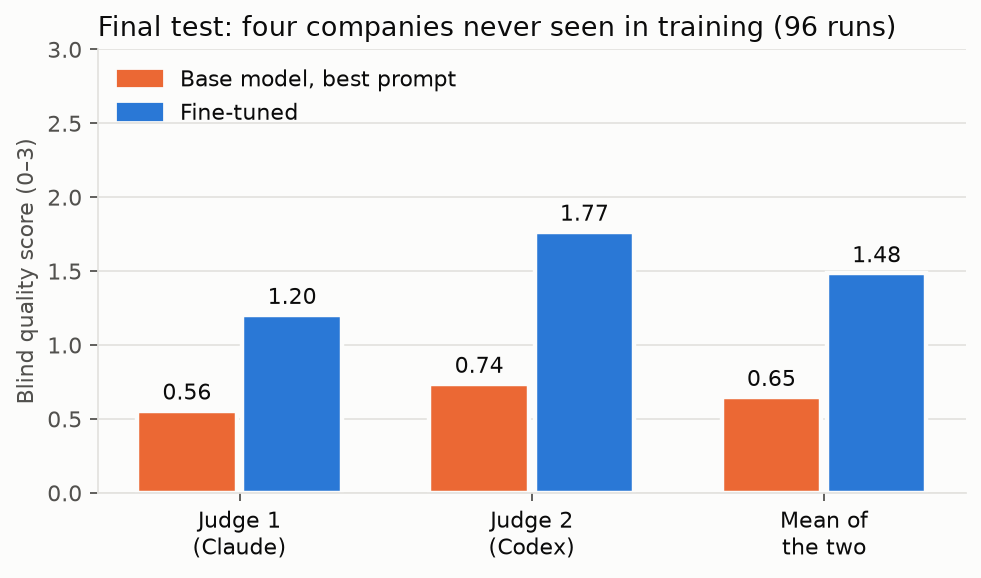
\includegraphics[width=\linewidth]{quality-light.png}\caption{Quality by judge.}\end{subfigure}
\begin{subfigure}{0.49\linewidth}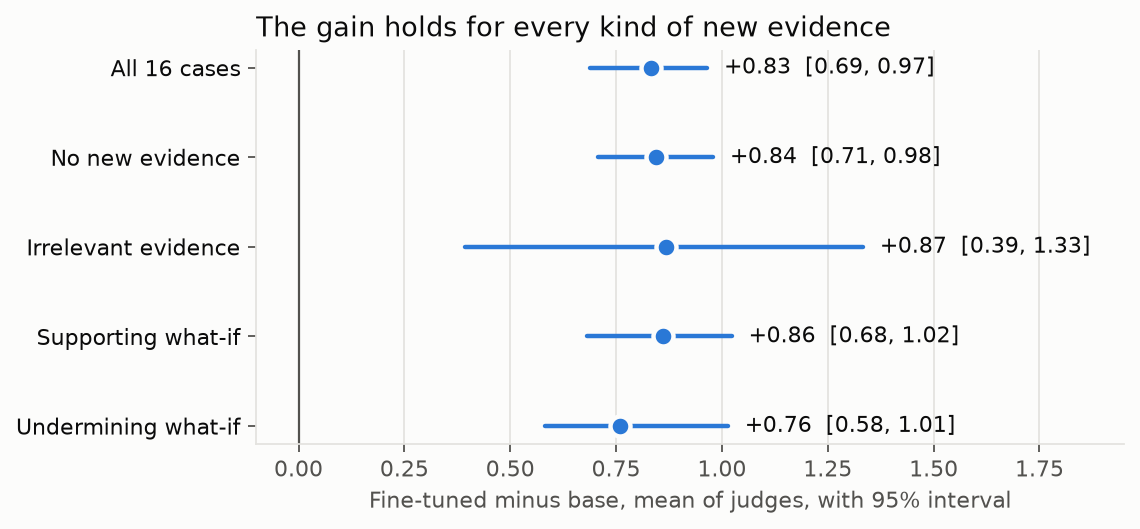
\includegraphics[width=\linewidth]{difference-light.png}\caption{Gain by kind of new evidence.}\end{subfigure}
\caption{Final test. Left: mean blind score per arm and judge. Right: fine-tuned minus base by kind of new evidence,
with 95\% intervals.}
\label{fig:final}
\end{figure}

\paragraph{By dimension.} \Cref{tab:dims} shows that the largest gains are in framing, causal mechanism and distinct
theories, the parts of the procedure the environment shapes most directly. Evidence judgement, experiment design,
revision and the recommendation improve but remain the weakest.

\begin{table}[H]\centering\small
\caption{Mean score per dimension, base $\to$ fine-tuned.}\label{tab:dims}
\begin{tabular}{@{}lcc@{}}
\toprule
Dimension & Claude & Codex\\
\midrule
Problem framing & 1.00 $\to$ 1.63 & 1.00 $\to$ 2.90\\
Causal mechanism & 0.92 $\to$ 1.44 & 1.15 $\to$ 2.63\\
Distinct theories & 0.57 $\to$ 1.60 & 0.98 $\to$ 2.56\\
Assumptions and predictions & 0.92 $\to$ 1.73 & 1.27 $\to$ 2.13\\
Evidence judgement & 0.17 $\to$ 0.79 & 0.40 $\to$ 1.17\\
Seeking challenge & 0.62 $\to$ 1.04 & 1.13 $\to$ 1.79\\
Experiment design & 0.40 $\to$ 0.98 & 0.40 $\to$ 1.08\\
Revision & 0.23 $\to$ 0.94 & 0.03 $\to$ 0.81\\
Recommendation & 0.09 $\to$ 0.58 & 0.08 $\to$ 0.58\\
\bottomrule
\end{tabular}
\end{table}

\paragraph{Beliefs.} Of the fine-tuned runs that stated a belief about the affected theory both before and after a
what-if, 6 of 6 moved in the allowed direction (3 undermining, 3 supporting) and none the wrong way; two runs lacked one of
the two statements. The base model stated no such pair.

\subsection{Cost}
A fine-tuned investigation reads about 121{,}700 prompt tokens and writes about 2{,}900, in 66 seconds on one A100 slice
(54 investigations per GPU hour). At the October 2026 median rental price of \$1.76 per hour that is \$0.032 per
investigation (\$0.016 at the lowest price, \$0.068 at a hyperscaler's). A measured control of Claude Opus 5.5 on the same
task cost \$0.248 per investigation, and the same token counts at Opus list prices would cost \$0.544. The comparison is
of cost, not quality: Opus was not run on the final test.

\section{Diagnosis: what still fails, and why}\label{sec:diagnosis}

\paragraph{Unfinished runs.} 20 of the fine-tuned model's 48 final-test runs ended before a recommendation. Nine reached
the turn limit, eight of them rereading the same few sources (19 to 30 reads of 4 to 10 sources). Eleven stopped after
repeated refusals, seven of them finish calls that cited only the simulated what-if, which the rules forbid (an eighth
such run reached the turn limit), and the rest repeated searches and assessments.

\paragraph{Finished runs.} Of the 28 finished runs, the experiment check fails in 23. In 17 of them the case says no test
is warranted, so the right call was to decline, but the model proposed a test; in 6 the check read the predictions as
too similar, and in 5 of those 6 the predictions were in fact opposite comparisons that the check misreads (a known
flaw). Evidence classes fail in 13 and evidence kinds in 11.

\paragraph{The training data explains much of it.}
\begin{itemize}
  \item No training row targets \Tool{decline\_test}: in all 15 training cases with no test warranted that the teacher
        ran, the teacher proposed a test anyway. The student cannot imitate a decision it never saw.
  \item Directional what-if evidence is rare: 6 undermining and 2 supporting among 205 teacher investigations on training
        companies, against 103 irrelevant and 94 with none.
  \item Constrained generation capped short text fields at 240 characters and cut them mid-sentence: 132 of the 158
        training test designs and 23 of the 37 accepted final-test proposals have a decision rule stopped at the cap. The
        model was trained on incomplete decision rules.
  \item On Aquaporin, no run in either arm read the company's insolvency records, and all eleven finished fine-tuned runs
        recommend investing: searching for a company's current position before theorising about it is a missing habit.
\end{itemize}

\paragraph{Teacher and student fail differently.} The student fails the experiment check far more often than the
teacher (82\% against 39\%), and evidence classes more (46\% against 27\%); it fails invented numbers (21\% against 70\%)
and evidence kinds (39\% against 83\%) less. The case distributions differ, so this is not a matched comparison, but it
suggests the student learned the teacher's form better than some of its judgement.

\section{Iteration after the final test}\label{sec:iteration}
Everything in this section is development work, reported separately from the final test, which is unchanged.

\subsection{Environment changes}
We tried changes to the environment alone, on the six validation companies with three attempts each (45 runs per
configuration), under a rule written before the runs: a configuration replaces the current one only if it finishes more
runs and does not lower the mean confidence score (\cref{sec:app}).

\begin{table}[H]\centering\small
\caption{Environment configurations on development (45 runs each).}\label{tab:env}
\begin{tabular}{@{}lrrrrr@{}}
\toprule
Configuration & Finished & Repeated refusals & Turn limit & Misquotes & Confidence\\
\midrule
As evaluated & 24 & 17 & 4 & 35 & 2.21\\
Reread limit, source dates, stuck help, 60 turns & 23 & 22 & 0 & 7 & 2.17\\
\bottomrule
\end{tabular}
\end{table}

Refusing a third read of the same source removed the turn-limit loops but turned them into refused calls, which end a run
after four in a row, and help after two refusals did not rescue enough of them, so the configuration was not adopted.
Misquotes fell from 35 to 7; showing each source's date in the state is the likely cause, though it was not tested
separately. A configuration with source dates and stuck help but no reread limit, and one requiring three weighed sources
per theory, were registered and are running at the time of writing.

\subsection{Targeted teacher examples}
We then tried to fix the data gaps directly with targeted examples: states harvested from the student's own runs at the
test step, at rereading loops and at refused finishes, answered once by the teacher under instructions for the missing
skill, filtered by code gates and reviewed by a human before any could train. Three advisory reviews (by separate
language-model agents, each with a different lens, and by Gemini) found the first rounds' answers to be templates: test
arms that differed only in a message, rival theories the answer itself called unsupported, decision rules that jumped to
developing a product line, and facts attributed to a case's year from later sources. The gates were tightened (complete
fields, no message-only arms without a control, a bounded next step, the currency and sources of the case's time) and,
after the human review, agree with all six of the reviewer's decisions on the second round; of those six answers, two were
kept. A third round, and later targeted corrective examples, are reported in Section~\ref{sec:negative}.

\subsection{A second test set}
Because the four final-test companies have informed the diagnosis, a new claim needed new companies. A second held-out
set of twelve companies and 24 present-day cases was built with the same pipeline, frozen before any run, and run once
under the unchanged protocol. On the mean of the two judges the fine-tuned model scores 1.09 and the base model 0.57, a
paired difference of $+0.52$ [0.33, 0.70] with a case-cluster bootstrap (Claude $+0.41$ [0.24, 0.57], Codex $+0.63$
[0.43, 0.84]; Spearman 0.95 between the judges over all 144 runs). The fine-tuned model is higher for 10 of 12
companies, and it finishes 32 of 72 investigations against 2 of 72. The gain is smaller than on the first test
($+0.83$ there).

\subsection{Later systems: a second adapter and adapter switching}
Two systems were built after the frozen results and are labelled exploratory. Version~3 continues version~1 on rows
from a second teacher (DeepSeek V4-Pro, 3,611 rows from 144 replay-exact investigations). \emph{Dig then reason} uses
one server holding both adapters: version~1 writes the brief, framing and evidence-gathering turns, version~3 every
later turn. Both were judged blind together with the base model and version~1 by the same two judges (mean of the two;
case-cluster bootstrap):

\begin{center}
\begin{tabular}{lcc}
\toprule
Arm & Test set 2 (72 runs) & Final test (48 runs)\\
\midrule
Base, staged prompt & 0.56 & 0.61\\
Version 1 & 1.07 & 1.45\\
Version 3 & 1.48 & 1.35\\
Dig then reason & 1.43 & 1.44\\
\bottomrule
\end{tabular}
\end{center}

On test set 2 dig then reason is clearly above version~1 ($+0.36$ [0.22, 0.51]); on the final test it is level with it
($-0.01$ [$-0.20$, 0.18]), and version~3 alone is not distinguishable from version~1 either ($-0.10$ [$-0.27$, 0.05]).
Version~1 remains the evaluated model; dig then reason is the most consistent later system and is the demo's default.

\paragraph{Loop guards.} Most refused calls in the final-test runs of dig then reason were repeats (233 of 274: the
same search again, or a source already weighed for that theory), and four refusals in a row end a run. Three guards act
only at decoding, with no retraining and no environment check changed: the assessment tool offers, per theory, only
sources not yet weighed; a quote is chosen from the source's own sentences; and a call refused as an exact repeat is
sampled again (at most three times, every refused draw kept in the record). With the step-budget aid of
Section~\ref{sec:negative} added, judged blind by both judges against dig then reason as evaluated (exploratory, built
after every frozen result):

\begin{center}
\begin{tabular}{lcc}
\toprule
 & Development (45 runs) & Test set 2 (72 runs)\\
\midrule
Finished runs, as evaluated $\rightarrow$ guarded & 28 $\rightarrow$ 45 & 43 $\rightarrow$ 63\\
Refused calls per run & 5.2 $\rightarrow$ 3.1 & 6.1 $\rightarrow$ 3.5\\
Quality, as evaluated $\rightarrow$ guarded & 1.42 $\rightarrow$ 1.62 & 1.43 $\rightarrow$ 1.59\\
Difference [95\% interval] & $+0.19$ [0.10, 0.30] & $+0.16$ [0.05, 0.27]\\
\bottomrule
\end{tabular}
\end{center}

The gain holds for each judge alone on both sets. On test set 2 the budget aid adds nothing over the three guards
($+0.006$ [$-0.010$, 0.022]), and one company (Testo) scores lower with the guards under both judges. Unlike the
advice-style aids of Section~\ref{sec:negative}, these guards remove the failing action from what the model can
produce, rather than telling the model about it.

\section{What did not fix the remaining failures}\label{sec:negative}
After both tests we tried, on the development cases only, to repair version 1's remaining failures:
\begin{itemize}
  \item invented numbers;
  \item weak or missing experiments;
  \item wrong evidence kinds;
  \item recommendations that do not follow the evidence;
  \item loops of refused calls.
\end{itemize}
Every attempt had its decision rule fixed before it ran. None succeeded. The failures fall into two different kinds,
and we keep them apart.

\subsection{Runtime interventions: the trained model does not use what it is told}
Each of these changes the harness around the unchanged version 1 adapter. The evaluated runner and settings stay as
they are.
\begin{itemize}
  \item \textbf{Recovery controller.} We tested four aids: masking rereads, progress notes, step-budget awareness and
        citation repair. Budget awareness rescued 15 of 28 stuck checkpoints against 6 for the baseline, but most of
        the rescued finishes failed a check. End to end, over 45 paired runs, it changed 8 runs and left quality
        unchanged ($+0.006$ [$-0.017$, 0.031]). Most failed runs stop earlier, after four refusals in a row, where no
        late aid acts.
  \item \textbf{Evidence verification.} Before the final recommendation, the agent was shown which cited sources
        postdate the case, which numbers no cited source gives, and whether any weighed source supports its favoured
        theory. It could revise or answer ``insufficient evidence''. Over 45 paired runs it gave 19 unsupported
        recommendations against 20, the same validated completion, and no abstention. After 26 of 27 reviews the model
        immediately rewrote its text without new evidence work, and most findings survived.
  \item \textbf{Constrained, evidence-consistent position (``V1.1'').} Constrained decoding offered as the favoured
        theory only those the agent's own weighings support. This collided with an existing guard: a theory must be
        challenged before it can be stated as the position. Finishes fell from 24 to 14 and validated completion from
        3 to 1, so it was rejected under its fixed rule.
  \item \textbf{Novelty-first search (``V1-r'').} The same keyword ranking, but each search returned records the run had
        not yet been shown. It doubled the sources surfaced (17.4 against 8.8 per run), but the agent read as many,
        weighed fewer (2.2 against 3.0), and weighed a contradicting source in the same 2 of 45 runs. Validated
        completion fell from 3 to 0, and the hits were less relevant. It was rejected under its fixed rule.
\end{itemize}
Advice does not change a 3B model's behaviour when nothing in its training data showed that behaviour. Constraints
change behaviour, but they interact with the environment's other guards.

\subsection{Training data: the teacher's errors are in the student}
An audit of the 158 teacher investigations that trained version 1 found the teacher's own weaknesses:
\begin{itemize}
  \item 74\% of its recommendations use a number from no source;
  \item 38\% of its evidence kinds match the annotation, with \texttt{independent\_study} often given to encyclopedia,
        news and company-history text;
  \item in 74 of its 109 historical cases (68\%; 47\% of all 158 investigations) the recommendation cites a source
        published after the case date, and in a blind content sample about half of those quotes reveal later outcomes.
\end{itemize}
Version 1 reproduces the first two: invented numbers in 21\% and 31\% of its finished recommendations on the two test
sets, and kinds matching in 58\% and 46\%. The frozen test cases are present-day, so the dating problem cannot affect
their scores. The dossier annotation itself agreed with a blind relabelling on 45 of 60 records, with 5 more
defensible.

\textbf{Corrective distillation} tried to fix this with the same teacher. We took states where version 1 went wrong on
training companies, asked the teacher for the right next step, and kept only answers that passed provenance, exact
replay, split and family gates. Of 90 answers the gates accepted, an advisory substantive review rated 3 strong, and
spot checks confirmed its reasons: later-dated sources, wrong kinds, overstated support, and tests that varied only
the message. A structured format fixed the teacher's truncated test designs, but then it declined tests the cases
warrant. We had fixed a threshold of 30 strong examples across three families, including experiment design, before
training. Command A+ did not meet it. A hosted teacher (DeepSeek V4-Pro, with V4.1-Flash) then met it with 105
corrective rows, and version 2 was trained on top of version 1; on its development screen it finished 0 of 15 runs
against version 1's 7, and it was stopped.

\textbf{What this does and does not show.} It shows that filtering cannot remove errors the teacher makes
systematically, and that the student inherits them. It does not show that better training data would fail. A stronger
or human-corrected teacher for evidence judgement and experiment design remains the most direct next step, and it was
not tested.

\section{aemon: the agent as a product}\label{sec:app}
An agent that only exists in an evaluation harness is not useful to a manager. aemon runs the fine-tuned model (by default version~1 gathering the evidence and version~3 reasoning, with the
loop guards of Section~\ref{sec:results})
locally (FastAPI and React over a llama.cpp server) and is designed, after a review of how current research assistants
present long-running work, for readers who are not analysts.

\begin{itemize}
  \item \textbf{Answer first.} A finished investigation opens with the recommendation, a confidence label and score,
        the next step and what would change the answer, then four headline numbers, then the explanations compared,
        the test, the sources, and only then the full trace.
  \item \textbf{Numbers counted from the record.} Every chart is computed from the investigation's own record, never
        estimated: how likely each explanation was judged before and after new evidence (an arrow plot on the five-step
        scale), how many weighed sources support or contradict each explanation (diverging bars), the mix of
        independent sources and company claims, and the test's cost and duration against its budget.
  \item \textbf{A confidence score out of five.} One point for each of five plain checks: the leading explanation is
        judged likely or better; it is judged very likely; at least two independent sources support it; no independent
        source contradicts it; at least three sources were weighed for it. Five is High, three or four Moderate, two or
        fewer Low, and a draft written after a run stopped early is never more than Low. On the final test's 28 finished
        runs the score was 2 in 24 runs, 3 in two and 4 in two: the agent never judges its favourite very likely, and it
        weighs few independent sources, which is exactly what the iteration targets.
  \item \textbf{Follow-up questions grounded in the investigation.} A follow-up is answered by the base model (adapters
        off) from the investigation's record and source excerpts only, under a schema whose citations can name only
        sources in the record; ``Re-investigate with this'' reruns the investigation with the new information, files
        or links instead.
  \item \textbf{Steps a reader can follow.} The trace is shown as the seven steps a manager would recognise (understand
        the question, gather sources, list explanations, weigh the evidence, stress-test the favourite, design a test,
        recommend), each expandable to its actions and each action to exactly what was read, quoted or decided.
  \item \textbf{Investigations that do not die.} Runs keep going when the page is closed; every turn is saved, and
        after a restart unfinished runs resume by replaying their saved turns, each of which must reproduce its saved
        result. A run that stops early can be continued from where it stopped, and if it ends without a recommendation
        aemon writes a labelled draft from what it found.
  \item \textbf{Memory, projects, attachments and web search.} Notes about the person, the company or a project are
        given to the agent as context, never as evidence; attached files and links become quotable sources labelled as
        the person's own; an optional live web search saves every page it reads and labels it unchecked; a mind map
        shows every investigation; every result downloads as a PDF report.
\end{itemize}
None of these features is part of the evaluated setup; the reported results apply to the frozen configuration.

\section{Limitations}\label{sec:limits}
\begin{itemize}
  \item \textbf{Generalisation.} Four test companies, all business-to-business manufacturers asked the same family of
        question, support only a limited claim. The second test set addresses this partly; other industries and other
        kinds of strategic question remain untested.
  \item \textbf{Replications.} Three attempts per case at temperature 0 are close to repeats; the effective sample is
        nearer 16 cases than 48 runs, which is why the intervals resample whole cases. The cases are themselves 4
        companies with 4 variants of one question, identical until the what-if arrives; resampling whole companies
        widens the final-test interval to $[0.63, 1.05]$ (bootstrap) or $[0.44, 1.23]$ (cluster-robust $t$, 3 degrees of
        freedom), and test set 2's to $[0.29, 0.75]$ or $[0.25, 0.78]$. With 4 companies any interval is rough; all 16
        cases and all 4 companies are higher.
  \item \textbf{Judges.} Both judges are language models. They were qualified and agree closely on the order of runs,
        but not on the level (on the same fine-tuned runs, problem framing 1.62 from Claude and 2.90 from Codex), so the
        comparisons rest on the order and absolute scores mean little. They may share biases, and no strategy expert has
        scored the runs.
  \item \textbf{Absolute quality.} 1.48 of 3 is a large relative gain but a modest absolute score; 20 of 48 runs ended
        before a recommendation, and the recommendation, revision, experiment design and evidence judgement remain the
        weakest dimensions.
  \item \textbf{Comparators.} The comparison is with the same base model under its best prompt, which reads the full
        transcript: 25 of its 48 runs stop at the context limit, and a stage never reached scores 0. Comparing each pair
        only on the dimensions both runs were scored on gives $+0.92$ [0.83, 1.01] (test set 2: $+0.90$ [0.81, 0.99]), so
        the base model is weaker even on the stages it reaches (\texttt{reports/judge/robustness.json}). Neither the teacher nor
        a closed model was run on the final test for quality; Claude appears only in the cost comparison.
  \item \textbf{Beliefs and confidence.} Beliefs are the agent's own verbal scale, not calibrated probabilities, and the
        belief check tests direction only.
  \item \textbf{Sources and outcomes.} The dossier is fixed and curated, with short excerpts; what-if results are
        written by the case authors; no recommendation was checked against what a company later did, and no proposed
        test was run. The results measure the quality of the investigation, not whether its advice would pay off.
  \item \textbf{Training.} One training run and one seed; variance across runs is not measured. The training data has a
        known defect, the 240-character cut of test designs, and no example of declining a test.
  \item \textbf{Controls.} The scripted negative controls could not run on the held-out cases and are reported for
        development only.
  \item \textbf{Teacher errors in the training data.} The rows are valid, accepted calls, but their content carries
        the teacher's errors (Section~\ref{sec:negative}): invented numbers, wrong evidence kinds, overstated support,
        and, in historical training cases, sources published after the case date. The model reproduces the first two.
  \item \textbf{Our own instruments.} The mechanical experiment check is lenient: on development it passes 9 tests, 8
        of which fail stricter design screens. The evidence-kind annotation matches a blind relabelling on 75\% of records, 83\% counting defensible
        alternatives. Both are reported
        as they are, and the frozen numbers use them unchanged.
  \item \textbf{Mechanical validity.} Few runs pass every check: 1 of 48 on the final test and 4 of 72 on the second.
        The quality gains are measured by blind judges, not by mechanical validity.
\end{itemize}

\section{Conclusion}\label{sec:conclusion}
A small open model can learn a meaningful part of a disciplined strategy procedure from a larger model's tool-using
investigations, provided the environment makes the procedure executable and the data are filtered for exactness. On a
frozen test it framed problems better, built genuinely distinct causal theories, gathered and weighed quoted evidence and
finished far more investigations than its base model, at a fraction of the cost of a closed model. It did not learn what
its teacher rarely showed it: declining a test that is not worth its cost, responding to directional new evidence, and
writing complete decision rules, and it inherited the teacher's habits of unsupported numbers and loose evidence
labels. Neither runtime aids nor corrective examples from the same teacher repaired these, which places the remaining
gap in the quality of the supervision. A better teacher for evidence judgement is the next step. Equally important is how the result was obtained: an environment that refuses rather than trusts,
training data bound to its provenance, judges qualified before use, and a test frozen and run once.

\section*{Team and acknowledgements}
Hatem Saadallah and Nour Jennane, Master's students in artificial intelligence and AI researchers (team Two-eyed
Ravens). Built with AgentTune and AuditKIT (Lexsi Labs), Tiny Aya and Command A+ (Cohere), PEFT, TRL and llama.cpp.
Claude (Anthropic) and Codex (OpenAI) served as blind judges and as coding assistants; no Claude output was used as
training data.


\bibliographystyle{plainnat}
\bibliography{refs}

\appendix
\section{Reproducibility}\label{app:repro}
\begin{itemize}
  \item \textbf{Model.} Tiny Aya Global, revision af89d21; adapter sha256 740c4a9b\ldots; evaluated GGUF adapter sha256
        41794b57\ldots, byte-identical across three conversions and to the file gated.
  \item \textbf{Teacher.} Command A+ (05-2026), Q4\_K\_M GGUF in four parts, first part sha256 03cf0669\ldots; llama.cpp,
        4 slots of 16{,}384 tokens, reasoning budget 512 from 4 November.
  \item \textbf{Final test freeze.} Case digest dce26d4f\ldots; runner code d3aa608; job script 0377eae; llama.cpp
        context 12{,}288, 520 tokens per turn, 45 turns, 4 refusals in a row; base prompt \texttt{staged}, fine-tuned
        prompt \texttt{compact}; judge configuration judge-v1-two-backends-2; bootstrap 4{,}000 resamples, seed 20261106.
  \item \textbf{Code and data.} The environment, pipeline, training and evaluation code and the job scripts are in the
        public repository; the model, the dossier, the cases, the training rows, every evaluation run, the
        judge packets, both judges' scores and the reports are on Hugging Face, with a manifest of the sha256 of every
        private original and its published copy. Since 11 November the public dossier is byte-identical to the one the
        evaluated runs read.
\end{itemize}
\end{document}
